% !TeX root = ../main.tex
% Add the above to each chapter to make compiling the PDF easier in some editors.

\chapter{Neutral Atom Architecture}\label{chapter:neutralatom}
There are already an impressive amount of approaches for building a \ac{QC}.
All of them are based on different physical systems that manage the creation, connection and manipulation of qubits \parencite{Wintersperger_2023}.
Some of the most promising approaches are:
\section{DiVichenzo Criteria?}
\section{Prevalent Architectures}
\subsection{Superconducting Qubits}
This architecture uses superconducting resonant circuits, that apply microwave signals to control and read qubits. 

The strong sites are its very fast single- and two-qubit gates,
electronics that cover current needs have been around for a long time and have been well studied 
e.g. commercial microwave devices can be used in experiments,
an increase of qubit amount in moderate effort is possible, 
different types of qubits \ref{fig:superconducting} and parameters with easy coupling nature of qubits allow high designability.

The week sides are necessity in very low temperature to operate, strongly limited coherence times, 
crosstalk between qubits requires careful design, complex error correction mechanisms,
a qubit isn't true two-level system, thus unwanted transitions must be avoided during processing. 
\parencite{Huang_2020}.
\begin{figure}[htbp]
  \centering
    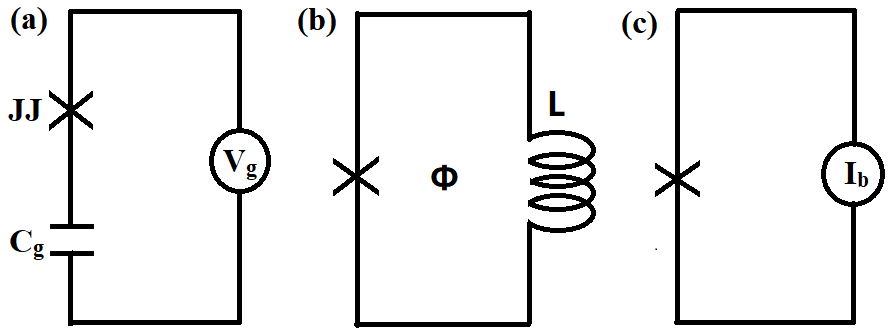
\includegraphics[width=0.8\textwidth]{figures/Superconducting.png}
    \caption{Three types of superconducting qubits circuit diagrams \parencite{Huang_2020}}
    \label{fig:superconducting}
    %referring by label \ref{fig:your-label}.
\end{figure}

\subsection{Photons}
Uses photons as qubits, computations are done via beam splitters, phase shifters, and detectors, that brings several points.

To advantages could be assigned operations with interference and entanglement by room temperatures,
low decoherence due to weak interaction with environment,
could be very helpful in the networks of quantum computers in the future.

Meanwhile, disadvantages include necessity in high-quality hardware to save and detect states,
complex error correction techniques, hard scaling
\parencite{romero2024photonicquantumcomputing}.

\subsection{Topological}
Encodes information non-locally using non-abelian anions such Majorana zero modes in topological superconductors 
or exotic materials. 
Logical gates are implemented via braiding operations that are inherently error-resistant.

Advantages are built-in topological protection that offers resilience to local noise, 
potentially reducing error correction complexity.

Disadvantages are hard experimental realization of stable non-abelian anions,
some operations are still theoretical or nascent.
\parencite{Lahtinen_2017, Zhang_2024}
\subsection{Ion Traps}
Uses positive ions such as Yb or Ca  placed in electromagnetic traps. 
Qubit states are encoded in stable electronic levels.

The strong sites are huge coherence time, that can be exceptionally long also without applying of decoupling techniques,
high fidelity of one-qubit and two-qubit gates, easy state preparation and readout.

The week side is non-triviality by scaling over fifty ions due to heating and crowding.
\parencite{Bruzewicz_2019}
\section{Neutral Atom}
The main considered physical architecture of this paper is \ac{NAQC}. 
This type of computer uses laser cooling and trapping techniques for neutral atoms and
optical or microwave pulses to manipulate quantum states.  
It offers long coherence times, scaling in 2D or even 3D,
and fair connectivities by long-range interactions (Rydberg states).
\subsection{Physical Hardware Implementation}
Consider \ref{fig:ColdAtomArchitecture} to have a schematic overview.
Neutral atoms such as Rubidium, Cesium or Strontium are placed in an ultra-high vacuum cell 
in a specific geometric arrangement often by optical tweezers. 
To work with them, they need to be cooled to very low temperatures.
The process of cooling is multistaged that especially involves Doppler cooling using a laser.
To place cooled atoms on fixed locations and keep them there a trap laser controlled by \ac{SLM} is employed.
With help of \ac{SLM} laser could be focused onto very small configurable points, this effect called optical tweezers.
\ac{SLM} could arrange atoms in 1D, 2D,or even in 3D configuration.
To move atoms there are another mobile traps controlled by \ac{AOD}.
\ac{AOD} implements the similar to \ac{SLM} function, but for mobile optical tweezers.
Then all of these electronic should be precisely calibrated to control process.

To perform actually computations laser and microwaves are employed, 
depends on executed gate used so-called Raman or Rydberg pulses, 
that could work locally or globally on arrangement of neutral atoms. 
\parencite{Schmid_2024_NeutralAtomBasics, Wintersperger_2023}
\begin{figure}[htbp]
  \centering
    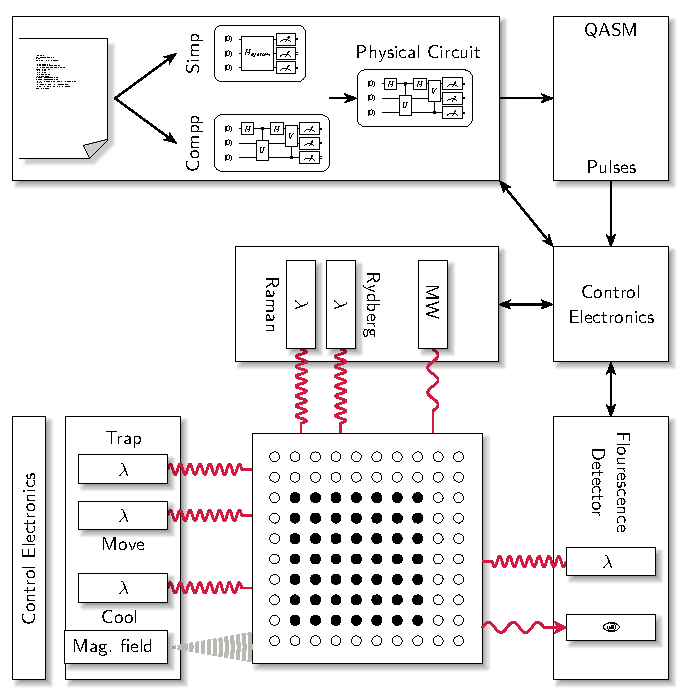
\includegraphics[width=0.8\textwidth]{figures/ColdAtomArchitecture.pdf}
    \caption{Schematic component overview of a cold atom quantum computer \parencite{Wintersperger_2023}}
    \label{fig:ColdAtomArchitecture}
\end{figure}

\subsection{Processing}
To use neutral atoms for performing quantum computations
encoding of qubit computation basis state need be found. 
These encoding should have a long coherence time and weak interaction with environment.
For Rubidium atom it is based on the spin of the furthest electron. 
Meanwhile, a Strontium implementation a nuclear spin of atom is used.

For implementing a one-qubit rotations operators two laser induced so-called Raman transition are used.
Target atom exposure to multiple photons and after that emits some another amount of energy,
what led to change of it state, by combining the duration, power and frequency of laser  
different direction and angles of rotation could be achieved.

For implementing a two-qubit gates a so-called Rydberg state is used. 
In this state an outermost electron has a very huge influence on other atoms' electrons in arrangement.
Thus, other atom cannot go in Rydberg state. This effect called Rydberg blockade.
An effective impact of this effect is a Controlled-Z gate.

Moreover, this effect allows implementing multiple-controlled Z-Gate directly on a hardware,
because Rydberg blockade influences not only on neighbor qubits but as a decreasing by distance field.
The strength of blockade obeys the proportion for small distances \(\frac{1}{|r|^3}\) and \(\frac{1}{|r|^6}\) for long.
Depending on a coefficient that accepted for blocking and interacting, 
different multiple-controlled Z-Gate are implemented.

Also, Rydberg blockade effect is used for long interactions between qubits within the acceptable range, 
it is with \ac{NAQC} possible to execute a two-qubit gate 
and do not require specifically place the atoms directly next to each other.

Nevertheless, if an interaction radius is too small for gate execution,
logical SWAP gates are considered to logically move qubit near to the target qubit.
But \ac{DPQA} could be based on neutral atoms. 
Hence, It makes possible to use physical moving of qubit in lattice, by moving it from \ac{SLM} to \ac{AOD} and back.
This process called shuttling.

For visualization of the described consider \ref{fig:NeutralAtomFeatures}.

\parencite{Wintersperger_2023, Philipp_Wondra_TUM_Thesis_for_Informatics.pdf}

\begin{figure}[htbp]
  \centering
    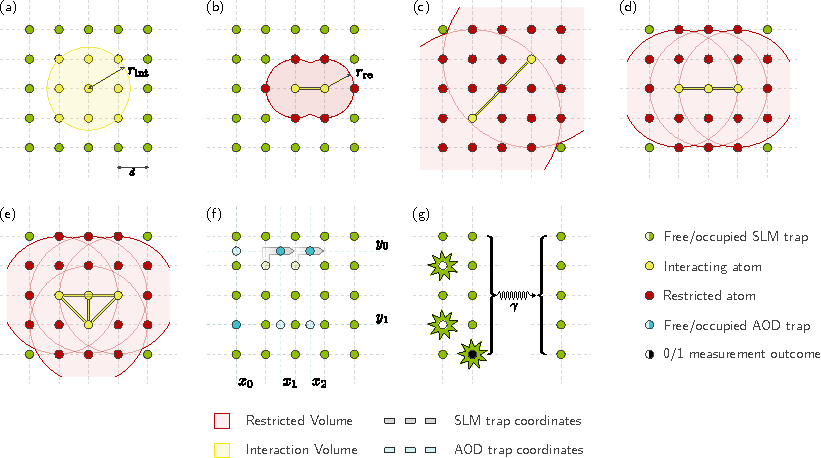
\includegraphics[width=0.8\textwidth]{figures/NeutralAtomFeatures.pdf}
    \caption{\textbf{Capabilities of the NAQC platform.} In this setup, atoms are arranged on a regular grid of \ac{SLM} traps, with a fixed distance denoted as $d$.
  \textbf{(a)} Rydberg blockade interaction: interacting gates can be performed to all qubits within this range.
  \textbf{(b)} Two-qubit gate: A gate can be applied between neighboring qubits but restricts the simultaneous execution of other entangling gates on nearby atoms.
   \textbf{(c)} Long-Range interactions: For gates with larger interaction radii, the restriction zones also expand, resulting in more restricted atoms.
  \textbf{(d)} CCZ gate with a line arrangement of the qubits. 
  According to \cite{Levine_2019} it is sufficient if the central atom interacts with both the outer qubits.
  \textbf{(e)} CCCZ gate 
  \textbf{(f)} Shuttling operation: \ac{AOD} (blue) enable the movement of atoms within the same column or row.
  \textbf{(g)} Additional NA capabilities, useful for future fault-tolerant computations. Not relevant for this work
   \parencite{Schmid_2024_NeutralAtomBasics}.
}\label{fig:NeutralAtomFeatures}
\end{figure}
